\documentclass[conference,12pt,onecolumn]{IEEEtran}
\usepackage[a4paper, left=2.5cm, right=2.5cm, bottom=2cm, top=2.5cm]{geometry}
\usepackage{graphicx}

\usepackage{makecell}
% Some very useful LaTeX packages include:
% (uncomment the ones you want to load)


% *** MISC UTILITY PACKAGES ***
%
%\usepackage{ifpdf}
% Heiko Oberdiek's ifpdf.sty is very useful if you need conditional
% compilation based on whether the output is pdf or dvi.
% usage:
% \ifpdf
%   % pdf code
% \else
%   % dvi code
% \fi
% The latest version of ifpdf.sty can be obtained from:
% http://www.ctan.org/pkg/ifpdf
% Also, note that IEEEtran.cls V1.7 and later provides a builtin
% \ifCLASSINFOpdf conditional that works the same way.
% When switching from latex to pdflatex and vice-versa, the compiler may
% have to be run twice to clear warning/error messages.






% *** CITATION PACKAGES ***
%
%\usepackage{cite}
% cite.sty was written by Donald Arseneau
% V1.6 and later of IEEEtran pre-defines the format of the cite.sty package
% \cite{} output to follow that of the IEEE. Loading the cite package will
% result in citation numbers being automatically sorted and properly
% "compressed/ranged". e.g., [1], [9], [2], [7], [5], [6] without using
% cite.sty will become [1], [2], [5]--[7], [9] using cite.sty. cite.sty's
% \cite will automatically add leading space, if needed. Use cite.sty's
% noadjust option (cite.sty V3.8 and later) if you want to turn this off
% such as if a citation ever needs to be enclosed in parenthesis.
% cite.sty is already installed on most LaTeX systems. Be sure and use
% version 5.0 (2009-03-20) and later if using hyperref.sty.
% The latest version can be obtained at:
% http://www.ctan.org/pkg/cite
% The documentation is contained in the cite.sty file itself.






% *** GRAPHICS RELATED PACKAGES ***
%
\ifCLASSINFOpdf
  % \usepackage[pdftex]{graphicx}
  % declare the path(s) where your graphic files are
  % \graphicspath{{../pdf/}{../jpeg/}}
  % and their extensions so you won't have to specify these with
  % every instance of \includegraphics
  % \DeclareGraphicsExtensions{.pdf,.jpeg,.png}
\else
  % or other class option (dvipsone, dvipdf, if not using dvips). graphicx
  % will default to the driver specified in the system graphics.cfg if no
  % driver is specified.
  % \usepackage[dvips]{graphicx}
  % declare the path(s) where your graphic files are
  % \graphicspath{{../eps/}}
  % and their extensions so you won't have to specify these with
  % every instance of \includegraphics
  % \DeclareGraphicsExtensions{.eps}
\fi
% graphicx was written by David Carlisle and Sebastian Rahtz. It is
% required if you want graphics, photos, etc. graphicx.sty is already
% installed on most LaTeX systems. The latest version and documentation
% can be obtained at:
% http://www.ctan.org/pkg/graphicx
% Another good source of documentation is "Using Imported Graphics in
% LaTeX2e" by Keith Reckdahl which can be found at:
% http://www.ctan.org/pkg/epslatex
%
% latex, and pdflatex in dvi mode, support graphics in encapsulated
% postscript (.eps) format. pdflatex in pdf mode supports graphics
% in .pdf, .jpeg, .png and .mps (metapost) formats. Users should ensure
% that all non-photo figures use a vector format (.eps, .pdf, .mps) and
% not a bitmapped formats (.jpeg, .png). The IEEE frowns on bitmapped formats
% which can result in "jaggedy"/blurry rendering of lines and letters as
% well as large increases in file sizes.
%
% You can find documentation about the pdfTeX application at:
% http://www.tug.org/applications/pdftex





% *** MATH PACKAGES ***
%
%\usepackage{amsmath}
% A popular package from the American Mathematical Society that provides
% many useful and powerful commands for dealing with mathematics.
%
% Note that the amsmath package sets \interdisplaylinepenalty to 10000
% thus preventing page breaks from occurring within multiline equations. Use:
%\interdisplaylinepenalty=2500
% after loading amsmath to restore such page breaks as IEEEtran.cls normally
% does. amsmath.sty is already installed on most LaTeX systems. The latest
% version and documentation can be obtained at:
% http://www.ctan.org/pkg/amsmath





% *** SPECIALIZED LIST PACKAGES ***
%
%\usepackage{algorithmic}
% algorithmic.sty was written by Peter Williams and Rogerio Brito.
% This package provides an algorithmic environment fo describing algorithms.
% You can use the algorithmic environment in-text or within a figure
% environment to provide for a floating algorithm. Do NOT use the algorithm
% floating environment provided by algorithm.sty (by the same authors) or
% algorithm2e.sty (by Christophe Fiorio) as the IEEE does not use dedicated
% algorithm float types and packages that provide these will not provide
% correct IEEE style captions. The latest version and documentation of
% algorithmic.sty can be obtained at:
% http://www.ctan.org/pkg/algorithms
% Also of interest may be the (relatively newer and more customizable)
% algorithmicx.sty package by Szasz Janos:
% http://www.ctan.org/pkg/algorithmicx




% *** ALIGNMENT PACKAGES ***
%
%\usepackage{array}
% Frank Mittelbach's and David Carlisle's array.sty patches and improves
% the standard LaTeX2e array and tabular environments to provide better
% appearance and additional user controls. As the default LaTeX2e table
% generation code is lacking to the point of almost being broken with
% respect to the quality of the end results, all users are strongly
% advised to use an enhanced (at the very least that provided by array.sty)
% set of table tools. array.sty is already installed on most systems. The
% latest version and documentation can be obtained at:
% http://www.ctan.org/pkg/array


% IEEEtran contains the IEEEeqnarray family of commands that can be used to
% generate multiline equations as well as matrices, tables, etc., of high
% quality.




% *** SUBFIGURE PACKAGES ***
%\ifCLASSOPTIONcompsoc
%  \usepackage[caption=false,font=normalsize,labelfont=sf,textfont=sf]{subfig}
%\else
%  \usepackage[caption=false,font=footnotesize]{subfig}
%\fi
% subfig.sty, written by Steven Douglas Cochran, is the modern replacement
% for subfigure.sty, the latter of which is no longer maintained and is
% incompatible with some LaTeX packages including fixltx2e. However,
% subfig.sty requires and automatically loads Axel Sommerfeldt's caption.sty
% which will override IEEEtran.cls' handling of captions and this will result
% in non-IEEE style figure/table captions. To prevent this problem, be sure
% and invoke subfig.sty's "caption=false" package option (available since
% subfig.sty version 1.3, 2005/06/28) as this is will preserve IEEEtran.cls
% handling of captions.
% Note that the Computer Society format requires a larger sans serif font
% than the serif footnote size font used in traditional IEEE formatting
% and thus the need to invoke different subfig.sty package options depending
% on whether compsoc mode has been enabled.
%
% The latest version and documentation of subfig.sty can be obtained at:
% http://www.ctan.org/pkg/subfig







% *** PDF, URL AND HYPERLINK PACKAGES ***
%
%\usepackage{url}
% url.sty was written by Donald Arseneau. It provides better support for
% handling and breaking URLs. url.sty is already installed on most LaTeX
% systems. The latest version and documentation can be obtained at:
% http://www.ctan.org/pkg/url
% Basically, \url{my_url_here}.




% *** Do not adjust lengths that control margins, column widths, etc. ***
% *** Do not use packages that alter fonts (such as pslatex).         ***
% There should be no need to do such things with IEEEtran.cls V1.6 and later.
% (Unless specifically asked to do so by the journal or conference you plan
% to submit to, of course. )


% correct bad hyphenation here
\hyphenation{op-tical net-works semi-conduc-tor}


\begin{document}
%
% paper title
% Titles are generally capitalized except for words such as a, an, and, as,
% at, but, by, for, in, nor, of, on, or, the, to and up, which are usually
% not capitalized unless they are the first or last word of the title.
% Linebreaks \\ can be used within to get better formatting as desired.
% Do not put math or special symbols in the title.
\title{Vehicle-to-Everything Communications (V2X) in 5G}


% author names and affiliations
% use a multiple column layout for up to three different
% affiliations
\author{\IEEEauthorblockN{Hugo Rummlinger, Frederik Schulz, Theo DDDDDDD, Anthony DDDDDDD}
\IEEEauthorblockA{Universitat Politecnica de Cataluna\\
Master of Science\\
5G Mobile Communication Systems}}


% make the title area
\maketitle

\begin{abstract}
In the abstract, you write 2-3 paragraphs which summarize the key parts of your report.
\end{abstract}


\IEEEpeerreviewmaketitle

\section{Papers Used \& How To Cite Them}
\begin{itemize}
\item V2X access technologies: Regulation, research, and remaining challenges [Cite: machardy2018] \cite{machardy2018}
\item Dedicated short-range communications (DSRC) standards in the United States [Cite: kenney2011] \cite{kenney2011}
\item Standards for vehicular communication---from IEEE 802.11p to 5G [Cite: festag2015]\cite{festag2015}
\item Ready to roll: Why 802.11 p beats LTE and 5G for V2x [Cite: filippi2016] \cite{filippi2016}
\item Heterogeneous Vehicular Networking: A Survey on Architecture, Challenges, and Solutions [Cite: zheng2015] \cite{zheng2015}
\item LTE-advanced in 3GPP Rel -13/14: an evolution toward 5G [Cite: lee2016] \cite{lee2016}
\item LTE for vehicular networking: a survey [Cite: araniti2013] \cite{araniti2013}
  \item Use cases, requirements, and design considerations for 5G V2X [Cite: boban2017] \cite{boban2017}
  \end{itemize}

\section{Introduction}
- Cooperative intelligent transportation systems (C-ITS) gained a lot of interest from different groups. V2X, short for Vehicle to Everything communication, is a specific case of ITS, dealing with wireless communication and coordination between vehicles and their environment.
- V2X can be taken in this paper to refer specifically to communication between overland road vehicles and other con- cerned entities, be they pedestrians, infrastructure, or other vehicles. \cite{machardy2018}
- Communication in V2X cases happens in a frequently changing vehicular ad-hoc networks (VANET)s, where nodes of the network leave and join the network at a specific location as frequently as the traffic floads. This VANET is supported by a static network. Nodes of this network a typically referred to as road side units (RSU), helping to coordinate non-static nodes communication traffic, distributing data and providing additional services \cite{machardy2018}.
- V2X technology tries to increase safety, efficiency and reduce economic costs of the current and future transportation system. \cite{machardy2018}

\section{Use-Cases}
\subsection{Vehicle-to-Vehicle}
\subsection{Vehicle-to-Infrastructure/Network}
\subsection{Vehicle-to-Person}

\section{Services}
- Services can be grouped into 4 major categories: Infotainment, Traffic Efficency, Cooperative Driving \cite{machardy2018}

- Infotainment:
- usually non-driving related topics.
- geo-realated advertisment
- messaging
- general media transfer, like internet services, netflix, etc.
- Infotainment services are characterized by relatively low min- imum latency requirements (latency on the order of 500 - 1000 ms, minimum transmission frequency on the order of 1 Hz) and throughput comparable to conventional mobile broadband services, up to around 80 Mbp \cite{machardy2018}

- Traffic Efficency:
- Broad application, generally tries to optimize traffic flow \cite{machardy2018}
- intersection timing handling
- real time route planning and changing, dependent on current/live situtation
- needs to exchange all information about current speed, current possition, as also destiny of a car
- usually not safety critical \cite{machardy2018}
- medium latency and throughput \cite{machardy2018}

-Traffic Safety:
- goal is to reduce frequency, severity of collision in our current transportation system, with regards vehicles involved.
- need for critical decision making, coping with non-standard behaviour of traffic participants, increase safety of especially, cyclist, pedestrians
- clearing roads for emergency cars
- Including not only crash prevention, but also knowing when an inavoidable crash will happen (pre-crash sensing) and taking all needed steps to reduce the impact of that event \cite{machardy2018}
- pre-crash sensing has highest requirements in this category: minimum round-trip latency of 50ms with 10Hz broadcast frequency \cite{machardy2018}.
- requirements for troughput will increase in the future, up to 700 mbps between vanet nodes estimated \cite{machardy2018}
- leads to a need for a high throughput, ultra reliable robust network.

\section{V2X in LTE Networks}
-  maybe  use \cite{araniti2013}
\subsection{Network}
Access Technologie from LTE point of vi

\subsection{Requirements}
Ffrom LTE point of view

\subsection{Services}

\section{Evolution from LTE to 5G}
- maybe use \cite{lee2016}

\subsection{Network}
Something about new infrstucture

\subsection{Requirements}


\subsection{Services}

\section{Other Access Technologies}
The following section deals with access technologies for V2X communication besides or in cooperation with cellular networks. We will only refer to the access technologies itself, if at all mentioning the eventually necessary infrastructure only briefly.
\subsection{Dedicated Short Range Communication}
Most scientific papers refer to dedicated short range communication (DSRC) as systems using IEEE 802.11p and  IEEE 1609 (WAVE) standards together for communication\cite{machardy2018}. Hereby the 802.11p standard allows for a setup of vehicular ad-hoc networks (VANET's) taking care of the physical (PHY) layer and the medium access (MAC) layer while the WAVE standard defines networking and some application related parts like security and authentication.
As an amendment to the Wi-Fi specification 802.11 defined by the IEEE organisation, 802.11p allows for inter device communication and is especially developed with V2X communication in mind. It facilitates the communication without the usual need for an basic service set (BSS, e.g. access point or something similar), allowing for D2D communication without a central coordinator \cite{machardy2018}. The standard itself does not define a specific operational frequencies, rather it defines the procedure of communication, leaving the choice of the used frequency to the authorities. As requirements for in V2X communication differ highly from typical Wi-Fi communication, 802.11p introduces a new medium access method called tiered contention multiple access (TMAC). This MAC technique allows for a prioritization of messages which is not possible with the typically used CSMA/CA technique \cite{machardy2018}. Especially for safety critical messages, relate to traffic safety like pre-crash sensing a prioritization of data flows is essential.
As with most wireless communications synchronization is needed for communication in DSRC \cite{kenney2011}. With the lack of an central coordination entity routing of multi-hop is a hard task in VANET's when mobility of nodes is high. Due to the fastly changing topology of the network, routes can be already obsoleted when found i\cite{machardy2018}. To which degree this affects communication depends heavily on the used routing protocol.
Another aspect in V2X communication is safety, as it is critical to have reliable communication partners. Users acting maliciously can spam the network or trying to insert wrong data into the network. DSRC uses a private key infrastructure for this aspect. Hereby a central authority distributes autonomous and temporal certificates to vehicles. Those are then used to sign messages. As malicious users can not be detected upfront there exist an entity, misbehaviour authority, which is entrusted with detecting malicious vehicles and adding them to a blacklist. For this system to work, vehicles need to regularly update their own list of blacklisted certificates. As this list can be relatively large, this system imposes requirements in terms of throughput and latency \cite{machardy2018}.

Summarizing it can be said, that DSRC allows for an low-end-to-end latency, a flexible organisation of nodes and relatively low cost for deployment in the V2X use-case. But it also entails a number of issues, including throughput problems in congestion situations, security issues and difficulties to handle non-line-of-sight communication \cite{machardy2018}. The U.S. Government of Transportation (USGOT) already specified DSRC for deployment. In the following this specification is used exemplary.

\subsubsection*{Standardization U.S. Government of Transportation}
- the following technical details are üall taken from the standardization from the USGOT and are not globally. But can be seen as examplary. for realisation for DSRC
- OFDMA uses a 10 MHz channel in DSRC
-  Testing of DSRC in the U.S. has focused on 10 MHz channels, based on the desire to support many parallel types of applications, and on physical testing that suggests this width is well suited to the delay and Doppler spreads likely to be encountered in the vehicular environ- ment \cite{kenney2011}
- for safety critival a braoder channel allows for less latency. But 20 MhZ channel have more noise.
- multiple mudolation rates
\begin{table}[h!]
  \begin{center}
    \caption{Modulation Options in DSRC 10 MHz OFDMA Channels. \cite{kenney2011}}
    \label{tab:table1}
    \begin{tabular}{ccccc}
      \textbf{\makecell{Modulation \\ Technique}} & \textbf{\makecell{Coded \\ Bit Rate\\ (Mbpcs)}} & \textbf{\makecell{Coding \\ Rate}} & \textbf{\makecell{Data Rate \\ (Mbps)}} &\textbf{ \makecell{Data Bits\\ per \\OFDMA Symbol}}\\
      \hline
      BPSK &6 & 1/2 &3 &24\\
      BPSK&6 &3/4&4.5&36\\
      QPSK&12 &1/2&6&48\\
      QPSK&12&3/4&9&72\\
      16-QAM&24&1/2&12&96\\
      16-QAM&24&3/4&18&144\\
      64-QAM&36&2/3&24&192\\
      64-QAM&36&3/4&27&216\\

    \end{tabular}
  \end{center}
\end{table}
- Forward error correction (FEC) coding is applied to the user bits, which reduces the effective user bit rate but also improves the probability of successful decoding
- opertes in the 5.9 GHz spectrum.
- Mac the traditional 802.11 functions of beacon- ing, synchronization, authentication, and association are not needed at the MAC sublayer for outside of contect bassic service set (OCB) communication
- Timing Advertisement (TA) frame, which can be used to announce information about the sender’s time source. needed to sync
- other functionalities are optionall and implemented at higher layers \cite{kenney2011}
- most communication probably single hop, therefore new layer 3 protocol\cite{kenney2011}
- also channel congestion is sicnificant concern for DSRC \cite{machardy2018}, efficency importatnt and new protocol goodd
- new Layer 3 protocol that is efficient for these 1-hop transmissions: the WAVE Short Message Proto- col (WSMP). Packets sent using WSMP are referred to as WAVE Short Messages (WSMs).
- authentication and encyrpion of messages is deinfed be WAVE and description ouf of scope.

\begin{figure} [h]
   \centering
  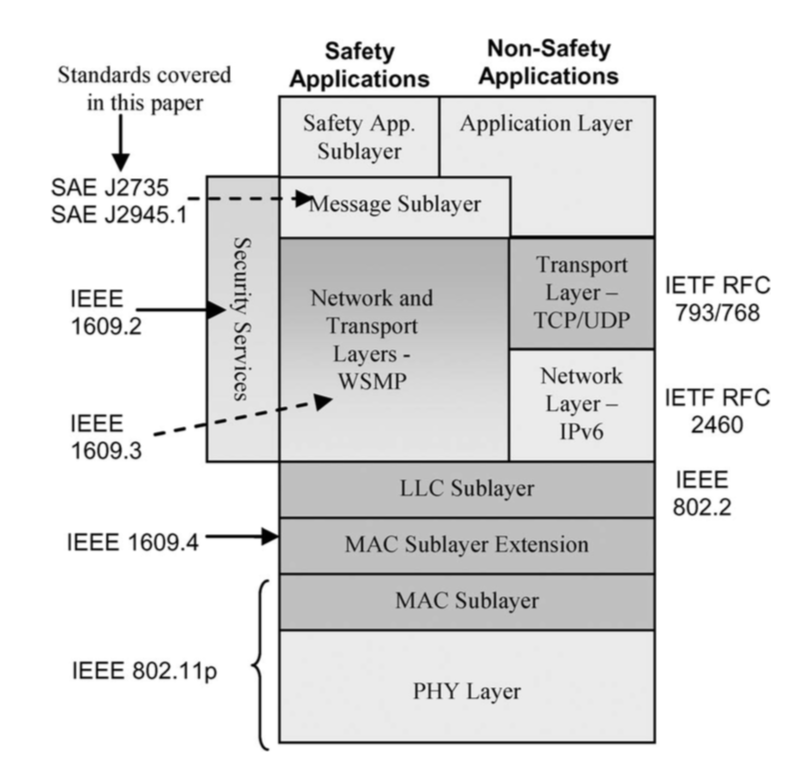
\includegraphics[width=0.5\linewidth]{_Graphics/layer_architecture_dsrc.png}
  \caption{Architecture of Layer Structure in DSRC (by USGOT). \cite{kenney2011}}
  \label{fig:boat1}
\end{figure}

\subsection{Visible Light Communication}
\subsection{Bluetooth}

\section{Results and Discussion}
\subsection{Cellular V2X versus DSRC}
- DSRC: need for a dense deployment to cope with line of sight problems, service degradation in congestion scenarios to name a few \cite{machardy2018}
- Who will pay for theses as IEEE 802.11p networks are typically not used outside, therefore networks typically do not have access control as cellular networks \cite{machardy2018} New use case for IEEE 802.11 protocol
- DSRC mandated standard by U.S. Department of Transportation (USDOT), European Telecommunications Standards Institute (ETSI), the European Committee for Standardization (CEN) [14], and the Association of Radio Industries and Businesses (ARIB) \cite{machardy2018}
- Cellular V2X (C-V2X) Compared to DSRC, these technologies offer a number of advantages, including a much larger coverage area, pre-existing infras- tructure, deterministic security and QoS guarantees, as well more robust scalability \cite{machardy2018}
- C-V2X has on negative side: Centralized architecture, higher price for network, higher end-to-end-latency!, dependency on network connectivity \cite{machardy2018}
- Latency is a major obstacle for C-V2X deployment. Services with high need for time sensitivity, e.g. cooperative platooning or pre-crash sensing need low latency \cite{machardy2018}
- Relate here somehow to Ultra Reliable Low Latency stuff from lecture.
- How is price determined in DSRC?
- Dependency of network connectivity should be able to be done by D2D sidelink without eNB or gNB beeing available. Source here.
- Would D2D sidelink also solve latency issues?
- evelopment of a Channel Congestion Control
algorithm, especially for the safety channe \cite{kenney2011}

\begin{table}[h!]
  \begin{center}
  \caption{Summary of Challenges for C-V2X and 802.11p-based DSRC. \cite{machardy2018}}
    \label{tab:table1}
    \begin{tabular}{lll}
      \textbf{\makecell{KPI}} & \textbf{\makecell{802.11p-based DSRC}} & \textbf{\makecell{Cellular V2X}} \\
      \hline
      \textbf{Latency}&{\tiny \makecell*[{{p{6.5cm}}}]{Not a cause for concern for 802.11p-based DSRC under normal operating conditions. An elevated packer error rate and the consequent need to retransmit messages can cause increased latency under sub-optimal conditions}}&{\tiny \makecell*[{{p{6.5cm}}}]{When operating through infrastructural nodes (e.g. eNB,EPC), processing delay is potentially problematic. Sidelink D2D and the provision of local edge resources are potential solutions to the problem of high latency}}\\
      \textbf{Capacity}&{\tiny \makecell*[{{p{6.5cm}}}]{Vehicular traffic congestion (several hundred vehicles within a 300m radius) can quickly cause high channel congestion and severely impact packer error rate. A potential path toward solving congestion issues may lie in improved congestion control schemes and controlling rate of transmissions. Optimal data-rates in the ballpark of 6 to potentially 27 Mbps are troublingly low, and may be insufficient to support many forthcoming V2X applications}}&{\tiny \makecell*[{{p{6.5cm}}}]{Depending on the size of the cell, frequent unicast transmissions via eNB from hundreds of vehicles can cause significant congestion. Using eMBMS or sidelink D2D may solve this problem. 5G aims to support data-rates measured in Gbps, which should be sufficient for all considered V2X applications}}\\
      \textbf{Coverage}&{\tiny \makecell*[{{p{6.5cm}}}]{LOS and relatively short communication range have implications for effective coverage for 802.11p-based DSRC. Communication through intermediate infrastructural nodes (e.g. RSUs) is one potential solution to the LOS communication problem.}}&{\tiny \makecell*[{{p{6.5cm}}}]{Coverage, particularly in mountainous and rural areas, can be inconsistent. Sidelink D2D is one potential solution to providing ubiquitous V2V coverage.}}\\
      \textbf{Security}&{\tiny \makecell*[{{p{6.5cm}}}]{Due to its ad-hoc nature, DSRC is vulnerable to a number of potential attacks on availability, authenticity, confidentiality and integrity. Some of these problems may be ameliorated by the implementation of vehicular private key infrastructure and decentralized misbehaviour detection, but many theoretical attacks, like vehicular worms and wormhole attacks, remain hard to defend against.}}&{\tiny \makecell*[{{p{6.5cm}}}]{Cellular V2X, the outgrowth of a centralized and long-commercialized communications technology, is somewhat less vulnerable to many security problems. Some attacks, particularly attacks on availability like jamming, remain difficult to defend against.}}\\
      \textbf{Privacy}&{\tiny \makecell*[{{p{6.5cm}}}]{The use of temporary pseudonymous certificates for authentication V2V communication provide a measure of privacy for DSRC nodes. Sophisticated eavesdropping and data interception may still pose a risk to driver privacy.}}&{\tiny \makecell*[{{p{6.5cm}}}]{The association of cellular communications with subscriber ID represents a potential compromise of UE privacy, particularly regarding authorities and network operators.}}\\
      \textbf{\makecell[l]{Infrastr.\\ \& Cost}}&{\tiny \makecell*[{{p{6.5cm}}}]{The lack of existing DSRC infrastructure and requirement for an extra DSRC-capable module in each vehicle stand to incur significant costs, both for municipal authorities and end users.}}&{\tiny \makecell*[{{p{6.5cm}}}]{The existing cellular infrastructure eases potential costs on municipal authorities, but high mobile data rates and cellular radios in each vehicle mean potentially high costs for end users.}}\\
    \end{tabular}
  \end{center}
\end{table}
\subsection{Bluetooth and VLC}
- several other technologies, including Bluetooth, satellite radio, and visible light communications have been considered for use for V2X applications. While each of these technologies has features which make it potentially promis- ing, each also has some unavoidable limitations, as covered in Section III-D, \cite{machardy2018}

\subsection{Heterogeneous Network}
- maybe something about our opinion if this solution is viable.
- good source \cite{zheng2015}
- Choice of wireless technology need not be an either-or proposition; many analyses have shown that a het- erogeneous solution can outperform either technology alone \cite{machardy2018}

\subsection{Standardization}
- While much of the technology involved in V2X communi- cation has been well-coordinated internationally, a number of regional differences have arisen. One of the most pointed dif- ference between the U.S. and EU V2X standards are the mes- sage sets defined for communication between vehicles \cite{machardy2018}
- could be a problem for traveling, common standard would be necessary to enable easier production and easier traveling.
- For detailed message evaluation see \cite{machardy2018}.

\section{Conclusion}
The conclusion goes here.

%\section{Section to see how to insert Table, Graphic and List}
%\subsection{A Subsection with Some Bullet Points}
%If you want, you can put some bullet points.
%\begin{itemize}
%\item This is a bullet point:
%\item This is another bullet point.
%\end{itemize}

%\subsection{Some Equations}
%Here is an equation:
%\begin{equation}
%a+b=c.
%\end{equation}

%\subsection{Figures and Tables}

%\begin{figure} [h]
%   \centering
%  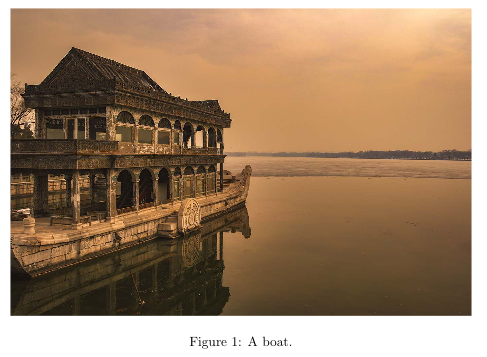
\includegraphics[width=0.5\linewidth]{_Graphics/boat1.png}
%  \caption{Example of a figure caption (the caption is placed below the figure).}
%  \label{fig:boat1}
%\end{figure}

%Figure \ref{fig:boat1} shows a boat.

%In the next page, I will create a table.
%\Begin{table}[h!]
%  \begin{center}
%    \caption{Table Caption.}
%    \label{tab:table1}
%    \begin{tabular}{l|l|r}
%      \textbf{Value 1} & \textbf{Value 2} & \textbf{Value 3}\\
%      $\alpha$ & $\beta$ & $\gamma$ \\
%      \hline
%      1 & 1110.1 & a\\
%      2 & 10.1 & b\\
%      3 & 23.113231 & c\\
%    \end{tabular}
%  \end{center}
%\end{table}

\bibliographystyle{IEEEtran} %the IEEtran file. You should not modify this file
\bibliography{IEEEabrv,references}

%references.bib is the name of the file where I wrote the references in .bib format


% that's all folks
\end{document}



%%% Local Variables:
%%% mode: latex
%%% TeX-master: t
%%% End:
